%
\section{Isothermal Two-Phase Flow}
This section ignores temperature effects and the partially saturated sample is treated as an immiscible two-phase system within the voids of the solid skeleton. In the pressure-pressure formulation the primary variables are (1) gas pressure $\asup{\pres}{g}$ and (2) capillary pressure $\asup{\pres}{c}$. In the pressure-saturation formulation the primary variables are non-wetting phase saturation ${\sat}^{nw}$ and wetting-phase pressure ${\pres}^{w}$. In the benchmarks shown here, both fluids are assumed incompressible.

\subsubsection*{Mass balance equation}
Consider two-phase flow in porous media, e.g liquid (denoted by $l$) and gas (denoted by $g$). For each phase in two-phase fluid flow, mass conservation is given by the following equation,

\begin{align}
\pD{}{t}\left(\poro S^g\dens_k^g+\poro S^l\dens_k^l\right)+\nabla \cdot \left( \FlxDf_k^g+\FlxDf_k^l\right)=Q_k,
\label{eq:massb}
\end{align}

where $S$ is saturation, $\dens$ stands for phase density, $\poro$ is the porosity, $\FlxDf$ is total flux. The subscript $k$ in equation (\ref{eq:massb}) denotes the component, e.g air ($k=a$) or water ($k=w$), within each phase, $\gamma=(g,l)$. For any phase $\gamma=(g,l)$, an advection vector ${{\FlxDf}_A}_k^{\gamma}$ and a diffusion vector  ${{\FlxDf}_D}_k^{\gamma}$ comprise the total flux, i.e,

\begin{align}
\FlxDf_k^{\gamma}={{\FlxDf}_A}_k^{\gamma}+{{\FlxDf}_D}_k^{\gamma}.
\label{eq:tflx}
\end{align}

According to Darcy's law, the advective part of the total flux may be written as

\begin{align}
{{\FlxDf}_A}_k^{\gamma}=-\dens_k^{\gamma}\dfrac{\perm \RelKa^{\gamma}}{\mu^{\gamma}}\left(\nabla \pres^{\gamma}-\dens^{\gamma} \mathbf g\right),
\label{eq:flx_dc}
\end{align}

where $\perm$ is the intrinsic permeability, $\RelKa^{\gamma}$ is the relative permeability of the phase, and $\mu^{\gamma}$ is the viscosity.

The diffusive part of the total flux is given by Fick's law

\begin{align}
{{\FlxDf}_D}_k^{\gamma}=-\poro \sat^{\gamma}  \dens^{\gamma} {\mathbb D}_k^{\gamma} \nabla \left(\dfrac{\dens_k^{\gamma}}{\dens^{\gamma}}\right),
\label{eq:flx_fk}
\end{align}

where $\mathbb D$ is the diffusion coefficient tensor. Since $\dens^{\gamma} = \dens_a^{\gamma}+\dens_w^{\gamma}$, we have

 \begin{align}
{{\FlxDf}_D}_w^{\gamma}+{{\FlxDf}_D}_a^{\gamma}=\mathbf 0
\label{eq:dufblc}
\end{align}

under the assumption ${\mathbb D}_a^{\gamma}  = {\mathbb D}_w^{\gamma} $.

Consider a water-air mixture. We expand the mass balance equation (\ref{eq:massb}) with the flux defined in equations (\ref{eq:tflx}) based upon the above equations (\ref{eq:tflx}, \ref{eq:flx_dc}, \ref{eq:flx_fk}). For the water component, the diffusive part of the total flux takes the form

\begin{align}
{{\FlxDf}_D}_w^{l}=-\poro \Sat^{l}  \dens^{l} {\mathbb D}_w^{l} \nabla \left(\dfrac{\dens_w^{l}}{\dens^{l}}\right),\quad
{{\FlxDf}_D}_w^{g}=-\poro \Sat^{g}  \dens^{g} {\mathbb D}_w^{g} \nabla \left(\dfrac{\dens_w^{g}}{\dens^{g}}\right).
\label{eq:flx_fkw}
\end{align}

Obviously, ${\mathbb D}_w^{l} = \mathbf 0$. Therefore, the mass balance equation for water component can be written as follows

\begin{align}
\pD{}{t} \left(\poro S^g\dens_w^g+\poro S^l\dens_w^l\right)-
\nabla \cdot \left[\dens_w^{l}\dfrac{\perm \RelKa^{l}}{\mu^{l}}\left(\nabla \pres^{l}-\dens^{l} \mathbf g\right)\right]\nonumber\\
-\nabla \cdot \left[\dens_w^{g}\dfrac{\perm \RelKa^{g}}{\mu^{g}}\left(\nabla \pres^{g}-\dens^{g} \mathbf g\right)\right] -
\nabla \cdot \left[\poro \Sat^{g}  \dens^{g} {\mathbb D}_w^{g} \nabla \left(\dfrac{\dens_w^{g}}{\dens^{g}}\right)\right] = Q_w.
\label{eq:massblq}
\end{align}

Since the capillary pressure $\pres^c$  is chosen as one of the two unknowns of equation (\ref{eq:massb}) and $S^g=1-S^l$, equation (\ref{eq:massblq}) becomes

\begin{align}
\poro (\dens_w^l -\dens_w^g)\pD{S^l}{t} +(1 -S^l)\poro \pD{\dens_w^{g}}{t} -
\nabla \cdot \left[\dens_w^{l}\dfrac{\perm \RelKa^{l}}{\mu^{l}}\left(\nabla (\pres^{g}-\pres^{c}) -\dens^{l} \mathbf g\right)\right]\nonumber\\
-\nabla \cdot \left[\dens_w^{g}\dfrac{\perm \RelKa^{g}}{\mu^{g}}\left(\nabla \pres^{g}-\dens^{g} \mathbf g\right)\right] -
\nabla \cdot \left[\poro \Sat^{g}  \dens^{g} {\mathbb D}_w^{g} \nabla \left(\dfrac{\dens_w^{g}}{\dens^{g}}\right)\right] = Q_w.
\label{eq:msblq}
\end{align}

Similar to the previous procedure, the diffusion part of the total flux of air component can be written as

\begin{align}
{{\FlxDf}_D}_a^{l}=-\poro \Sat^{l}  \dens^{l} {\mathbb D}_a^{l} \nabla \left(\dfrac{\dens_a^{l}}{\dens^{l}}\right),\quad
{{\FlxDf}_D}_a^{a}=-\poro \Sat^{g}  \dens^{g} {\mathbb D}_a^{g} \nabla \left(\dfrac{\dens_a^{g}}{\dens^{g}}\right).
\label{eq:flx_fka}
\end{align}

The density shift from air component to liquid ${\dens_a^{l}}$ is very small and can be omitted. Therefore, we can assume ${{\FlxDf}_D}_a^{l}\thickapprox0$. As a consequence, the mass balance equation for air component is derived:

$$\pD{}{t} \left(\poro S^g\dens_a^g\right) -$$
\begin{align}
\nabla \cdot \left[\dens_a^{g}\dfrac{\perm \RelKa^{g}}{\mu^{g}}\left(\nabla \pres^{g}-\dens^{g} \mathbf g\right)\right]-\nabla \cdot \left[\poro \Sat^{g}  \dens^{g} {\mathbb D}_a^{g} \nabla \left(\dfrac{\dens_a^{g}}{\dens^{g}}\right)\right] =Q_a.
\label{eq:massba}
\end{align}

Expanding the temporary derivative term of equation (\ref{eq:massba}) yields

$$-\poro \dens_a^g \pD{S^l}{t} + (1 -S^l)\poro \pD{\dens_a^{g}}{t}-$$
\begin{align}
\nabla \cdot \left[\dens_a^{g}\dfrac{\perm \RelKa^{g}}{\mu^{g}}\left(\nabla \pres^{g}-\dens^{g} \mathbf g\right)\right] -
\nabla \cdot \left[\poro \Sat^{g} \dens^{g} {\mathbb D}_a^{g} \nabla \left(\dfrac{\dens_a^{g}}{\dens^{g}}\right)\right] = Q_a.
\label{eq:msba}
\end{align}

The mass balance equations (\ref{eq:msblq}) and (\ref{eq:msba}) are exactly the same as described in \cite{SanPesSch:06}.

\subsubsection*{Pressure-pressure (pp) scheme}
Based on the description of isothermal two-phase flow above, (\ref{eq:msblq}) and (\ref{eq:msba}) can be modified in order to obtain governing equation for the isothermal two-phase flow in a porous medium. In this formulation primary variables are gas pressure $\asup{\pres}{g}$, and capilary pressure $\asup{\pres}{c}$.

The basic equations of the isothermal two-phase flow system are:

\begin{align}
\poro \dens_w \pD{S_w}{\pres_c} \dot\pres_c +
\nabla \cdot\left[\dens_w\dfrac{{\perm \RelKa}_{w}}{\mu_w}\left(-\nabla \pres^{g} +
\nabla{\pres}^{c} + \dens_w \mathbf g\right)\right] = Q_w
\end{align}
\begin{align}
- \poro \dens^a \pD{S_w}{\pres_c} \dot\pres_c+
\poro (1 -S_w)\left(\pD{\dens_a}{\pres^g}\dot\pres^g+\pD{\dens_a}{\pres_c}\dot\pres_c\right)+ \nonumber\\
\nabla \cdot \left[\dens_a\dfrac{{\perm \RelKa}_a}{\mu_a} \left(-\nabla\pres^{g} + \dens_a \mathbf g\right) \right] = Q_a
\label{eq:msbl_sim}
\end{align}

\subsubsection*{Pressure-saturation (pS) scheme}
Based on the description of the isothermal two-phase flow above, (\ref{eq:msblq}) and (\ref{eq:msba}) can be modified in order to obtain governing equation for the isothermal two-phase system. Primary variables of this formulation are wetting phase pressure $p_w$, and non-wetting phase saturation $S_{nw}$. The equations are simply algebraic manipulations of those in the previous section.

%-------------------------------------------------------------------------
%-------------------------------------------------------------------------

\subsection{Liakopoulos experiment}

\subsubsection*{Definition}
This benchmark is based on an experiment by Liakopoulus \cite{Lia:65} and is proposed by Lewis and Schrefler \cite{LewSch:98}(pp 167--174). The Liakopoulos test case is already described and used for unsaturated consolidation in Chapter 6. There you can find the complete problem definition.

The benchmark is simulated with different element types using the pressure-pressure scheme. The grids used in such simulations are illustrated in Fig. \ref{liak:grids}.

\begin{figure}[!tbh]
\begin{center}
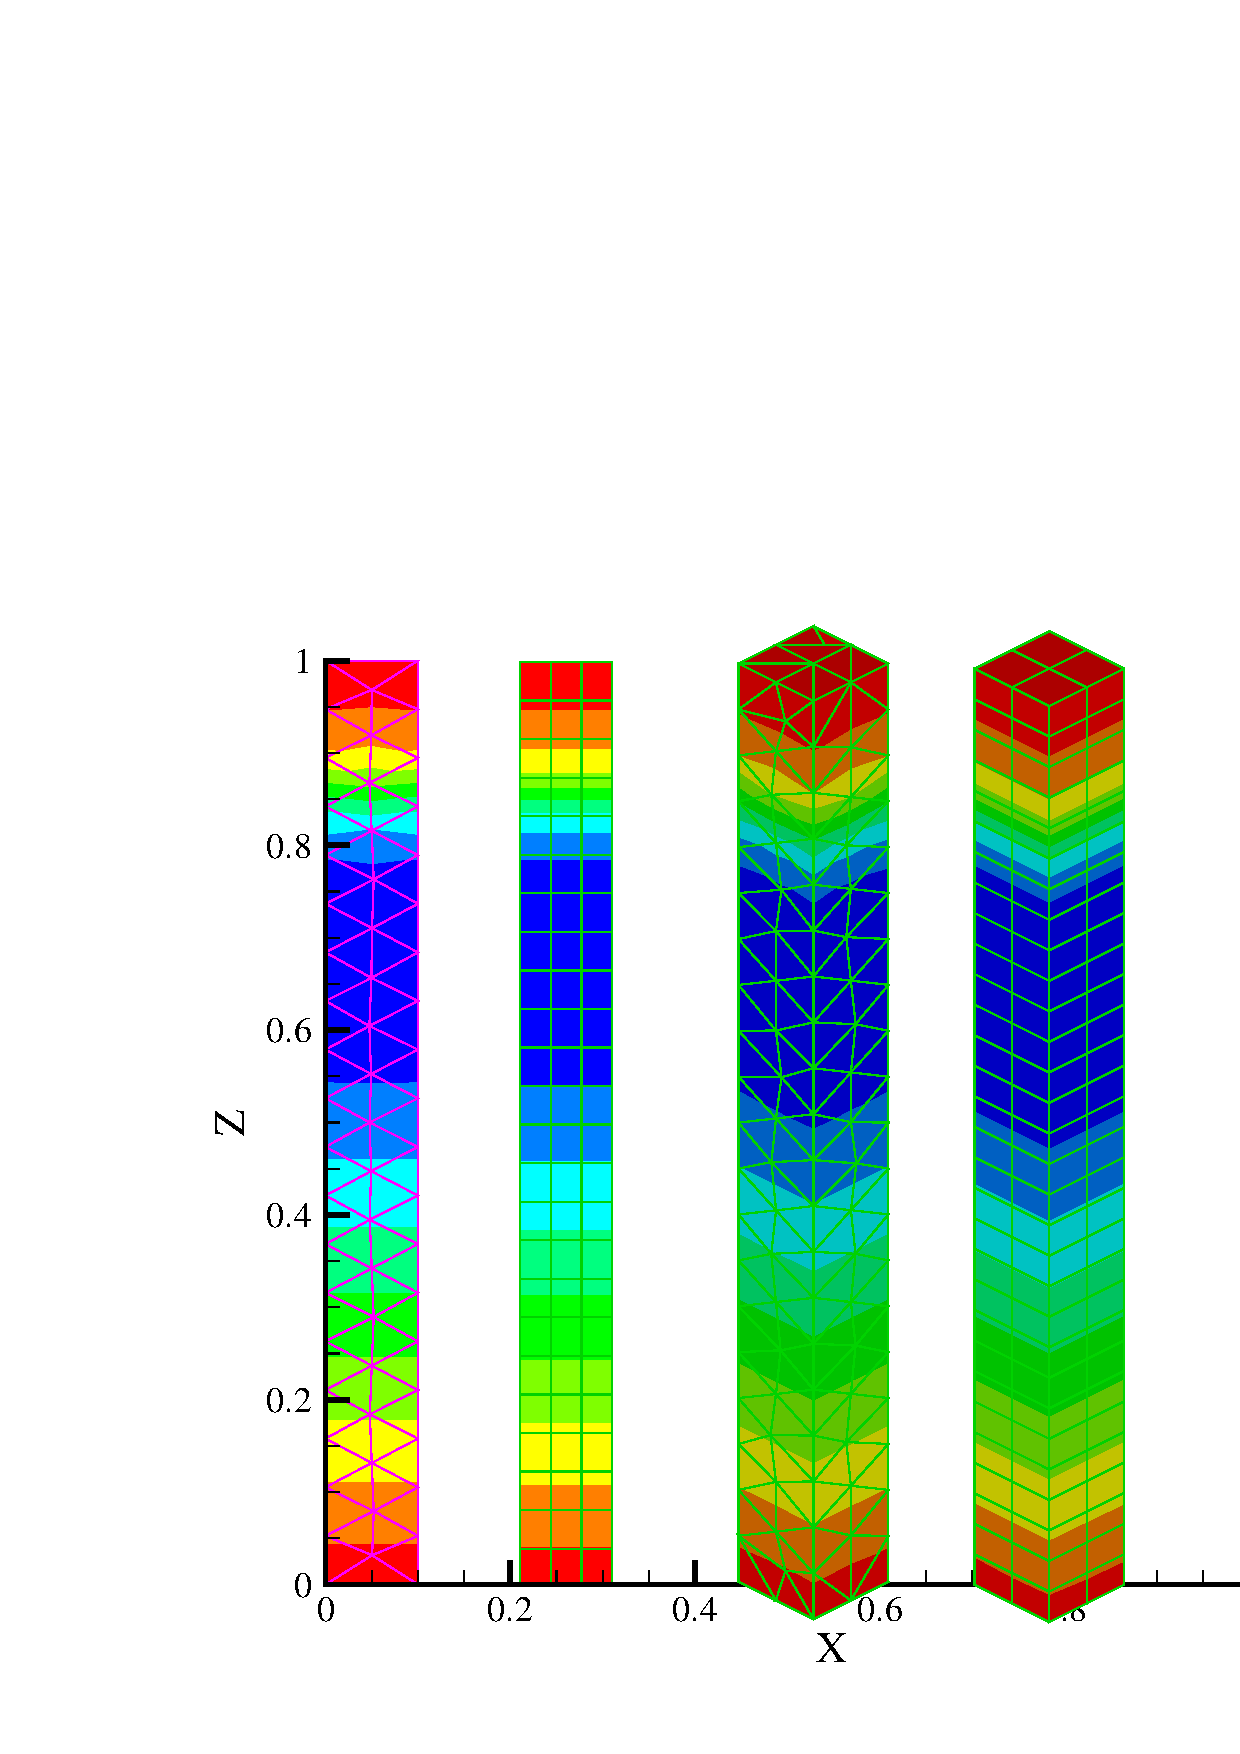
\includegraphics[scale=0.35]{chapter_13/figures/fig_13_1_1}
\end{center}
\caption{Grids with different element types for the Liakopoulos benchmark.}
\label{liak:grids}
\end{figure}

\subsubsection*{Results}
The temporal evolution of vertical profiles of primary variables (capillary and gas pressure) are given in Fig. \ref{liak:p_pc}. Fig. \ref{liak:p_sat} shows the vertical profiles for water saturation as a secondary variable. The results agree well with the findings by Lewis and Schrefler \cite{LewSch:98}.

\begin{table}[!htb]
\begin{tabular}{lccr}
\hline\noalign{\smallskip}
Property & Symbol & Value & Unit \\
\noalign{\smallskip}\hline\noalign{\smallskip}
Porosity & $n$ & -- & $2.975\times10^{-1}$ \\
Permeability & $\kappa$ & $ m^2$ & $4.5000\times 10^{-13}$ \\
Liquid dynamic viscosity &  $\mu_w$ & $Pa.s$ & $1.0000\times10^{-3}$ \\
Gas dynamic viscosity & $\mu_a$ & $Pa.s$ & $1.8\times10^{-5}$ \\
Liquid density &  $\rho_w$ &$kg.m^{-3}$ & $1.0000\times10^{3}$ \\
Gas density &  $\rho_a$ & $kg.m^{-3}$ & Ideal Gas Law's \\
Capillary pressure & $p^c$ & $Pa$ & Experimental Curve \\
Relative permeability & ${\kappa_{rel}}_{w}$ & -- & Experimenta Curve\\
Relative permeability & ${\kappa_{rel}}_{a}$ & -- & Brook-Corey functions \\
\noalign{\smallskip}\hline
\end{tabular}
\caption{Material parameters for the Liakopoulos problem.}
\end{table}

\begin{figure}[!tbh]
\begin{center}
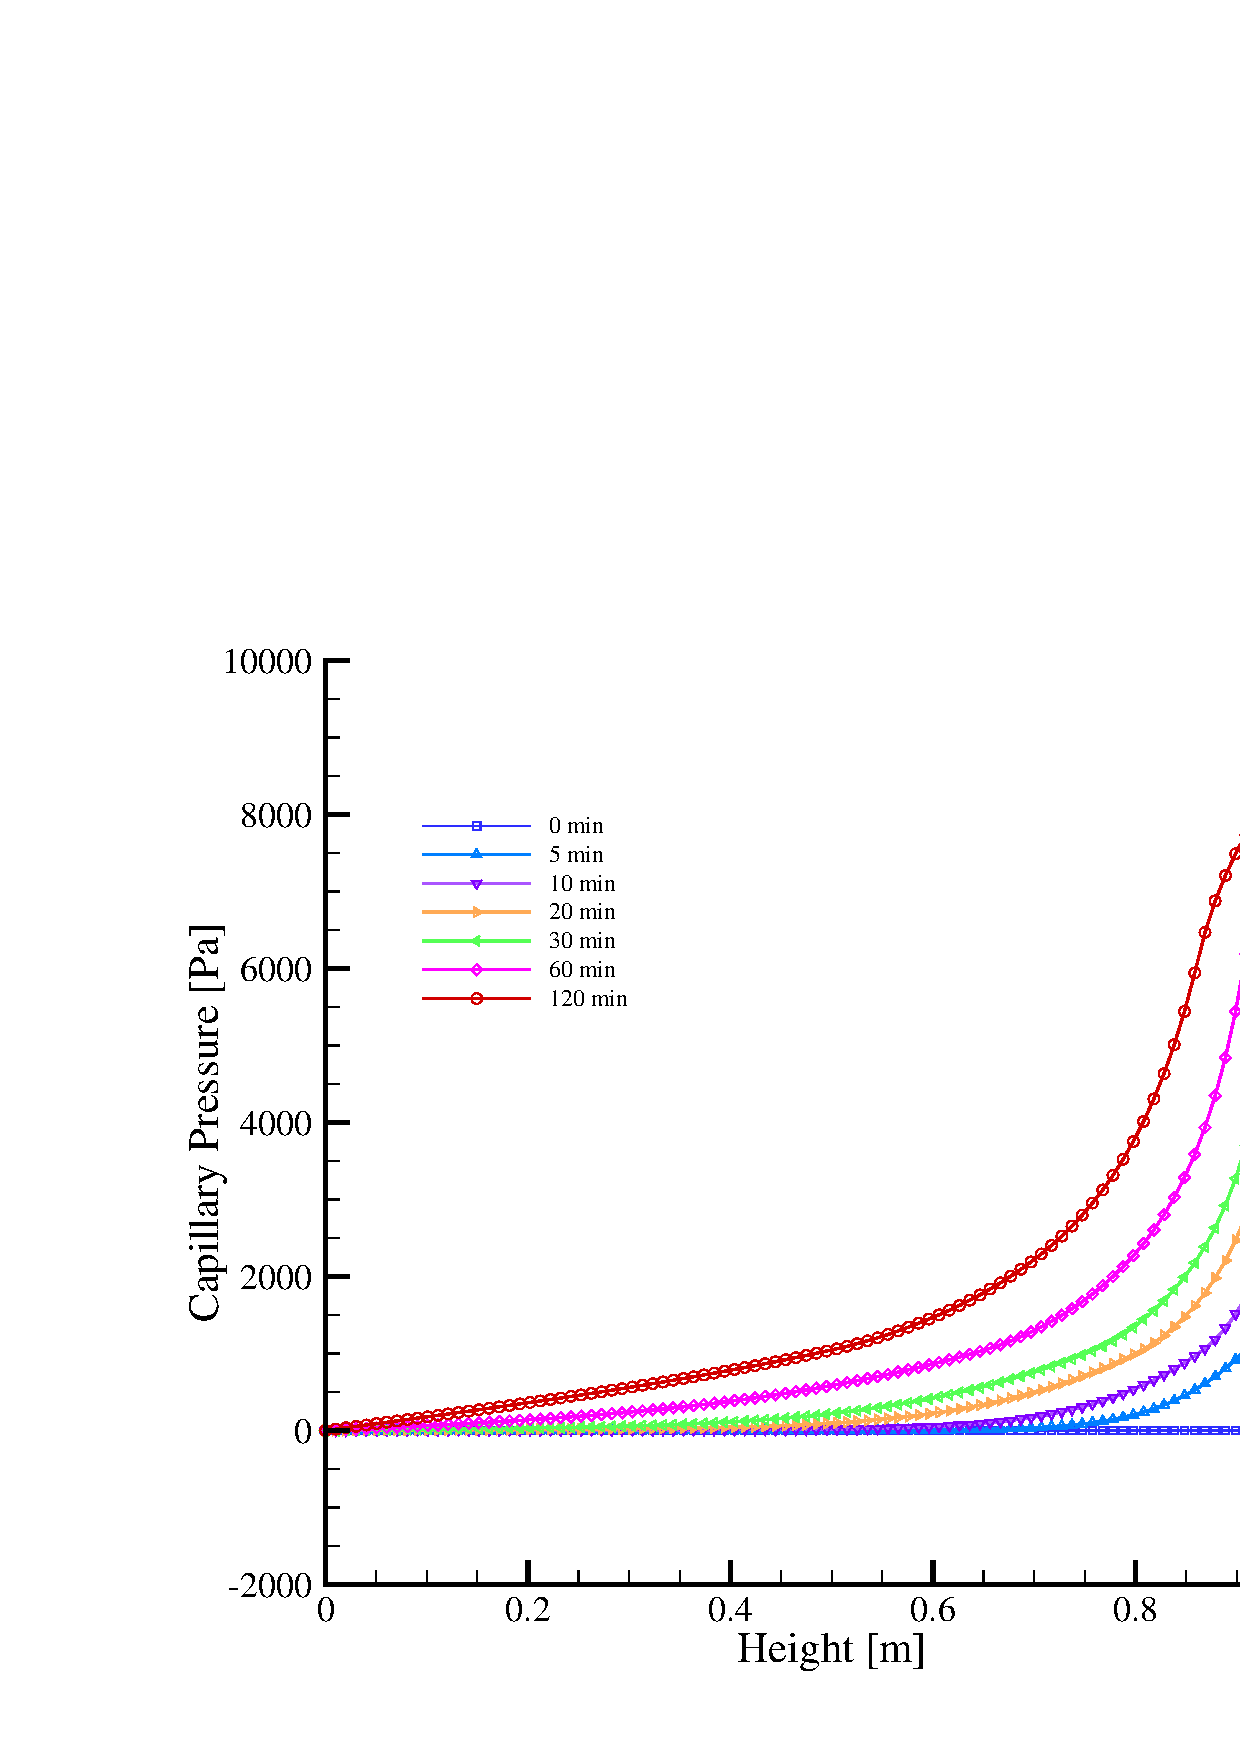
\includegraphics[scale=0.42]{chapter_13/figures/fig_13_1_2_a}
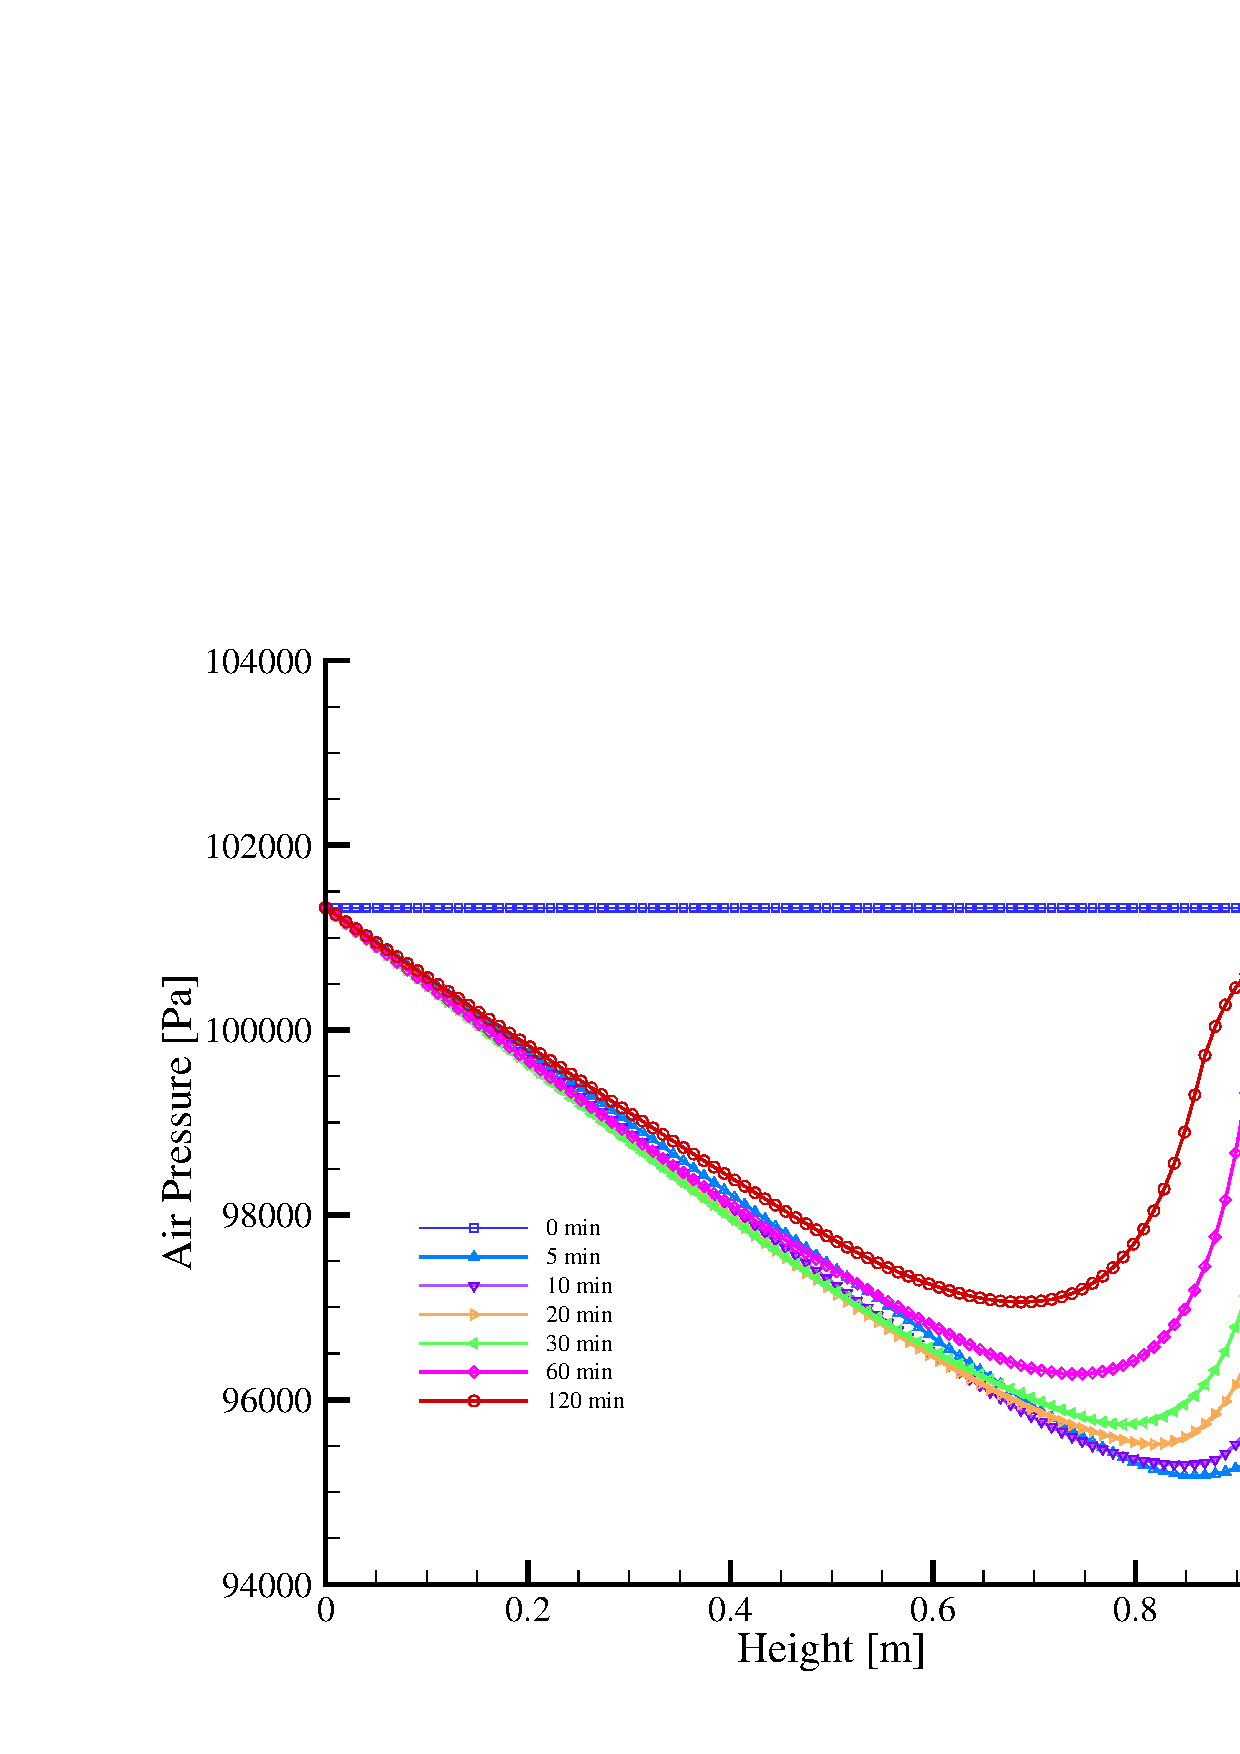
\includegraphics[scale=0.42]{chapter_13/figures/fig_13_1_2_b}
\end{center}
\caption{Vertical profiles of capillary (top) and gas pressures (bottom).}
\label{liak:p_pc}
\end{figure}

\begin{figure}[!tbh]
\begin{center}
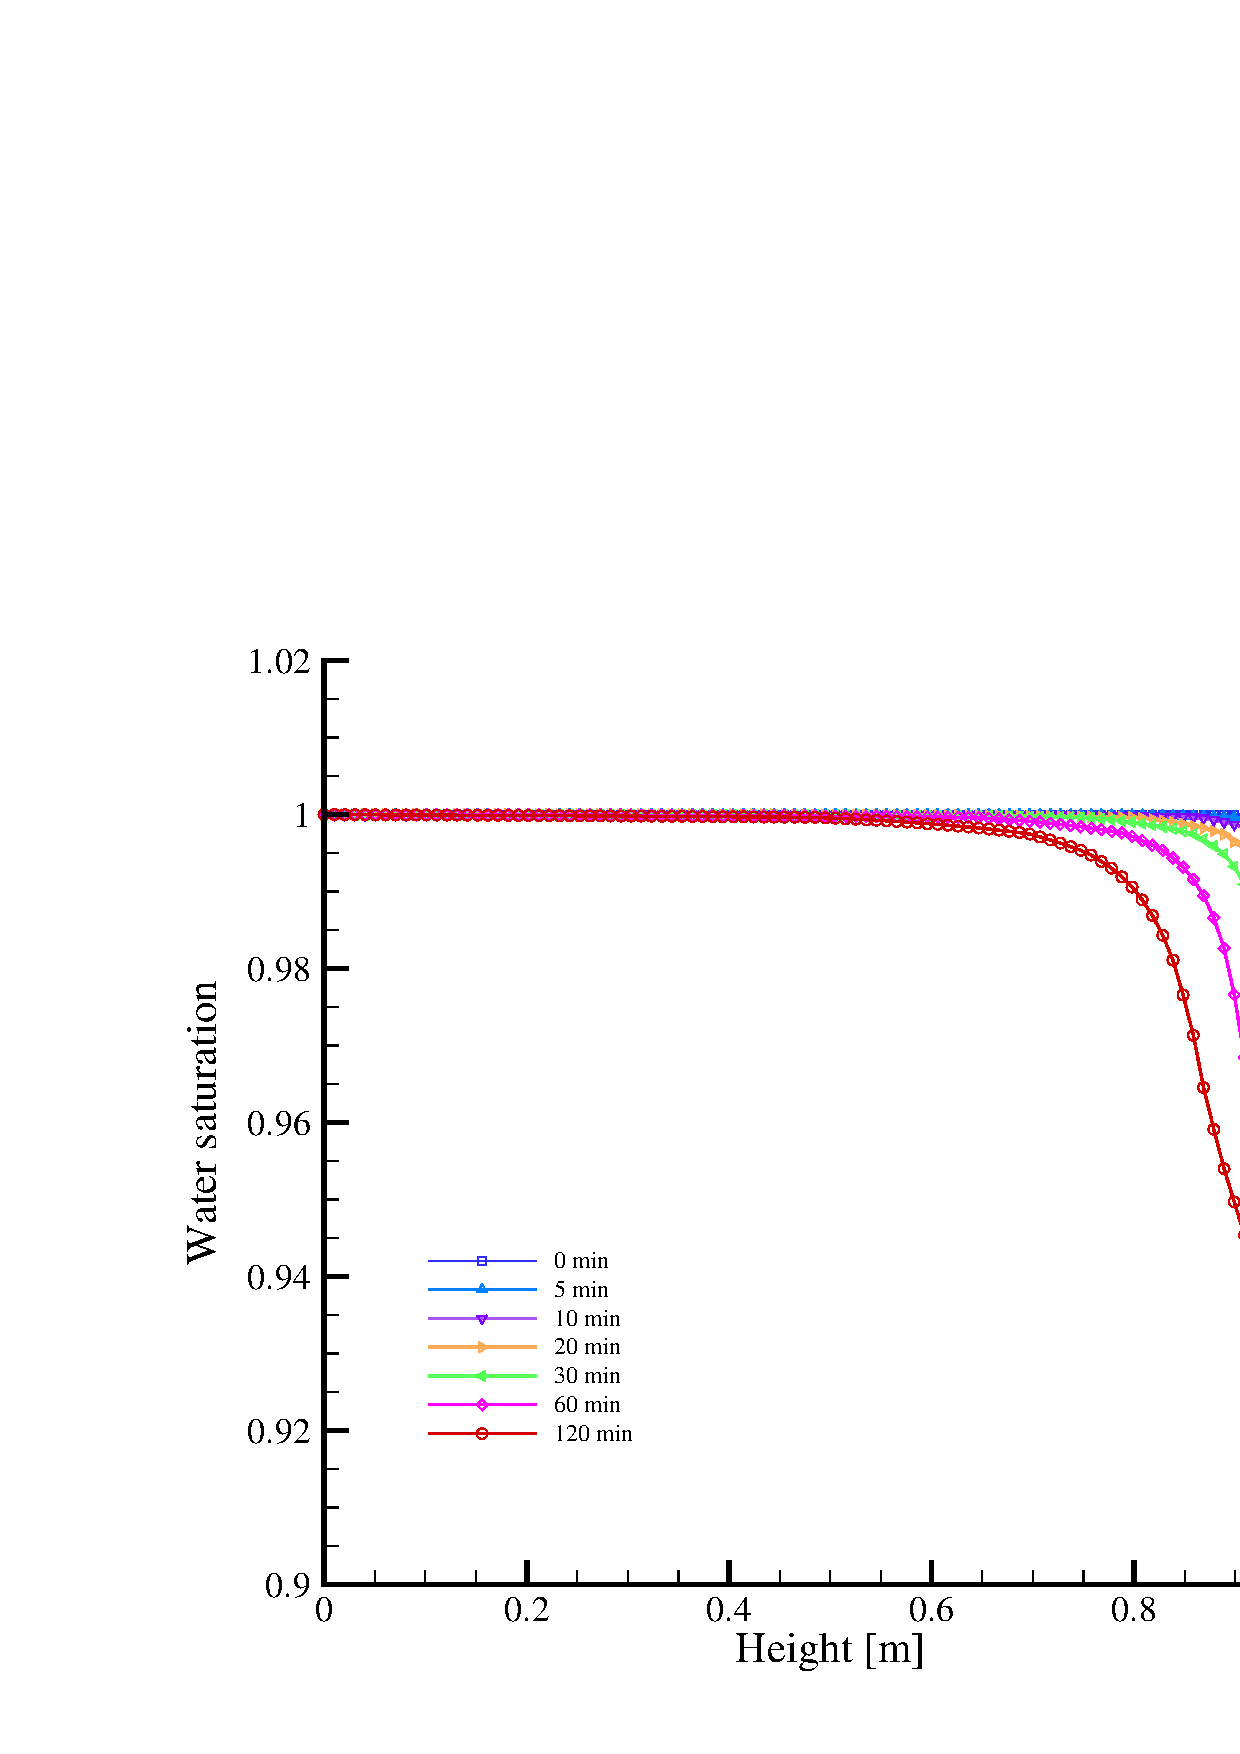
\includegraphics[scale=0.38]{chapter_13/figures/fig_13_1_3}
\end{center}
\caption{Profile of water saturation.}
\label{liak:p_sat}
\end{figure}

The results of the element test are depicted in Fig. \ref{liak:p_pce} for capillary pressure. A comparison if the results between the two-phase flow model and the Richards model can be found in Chapter 6. 

\begin{figure}[!tbh]
\begin{center}
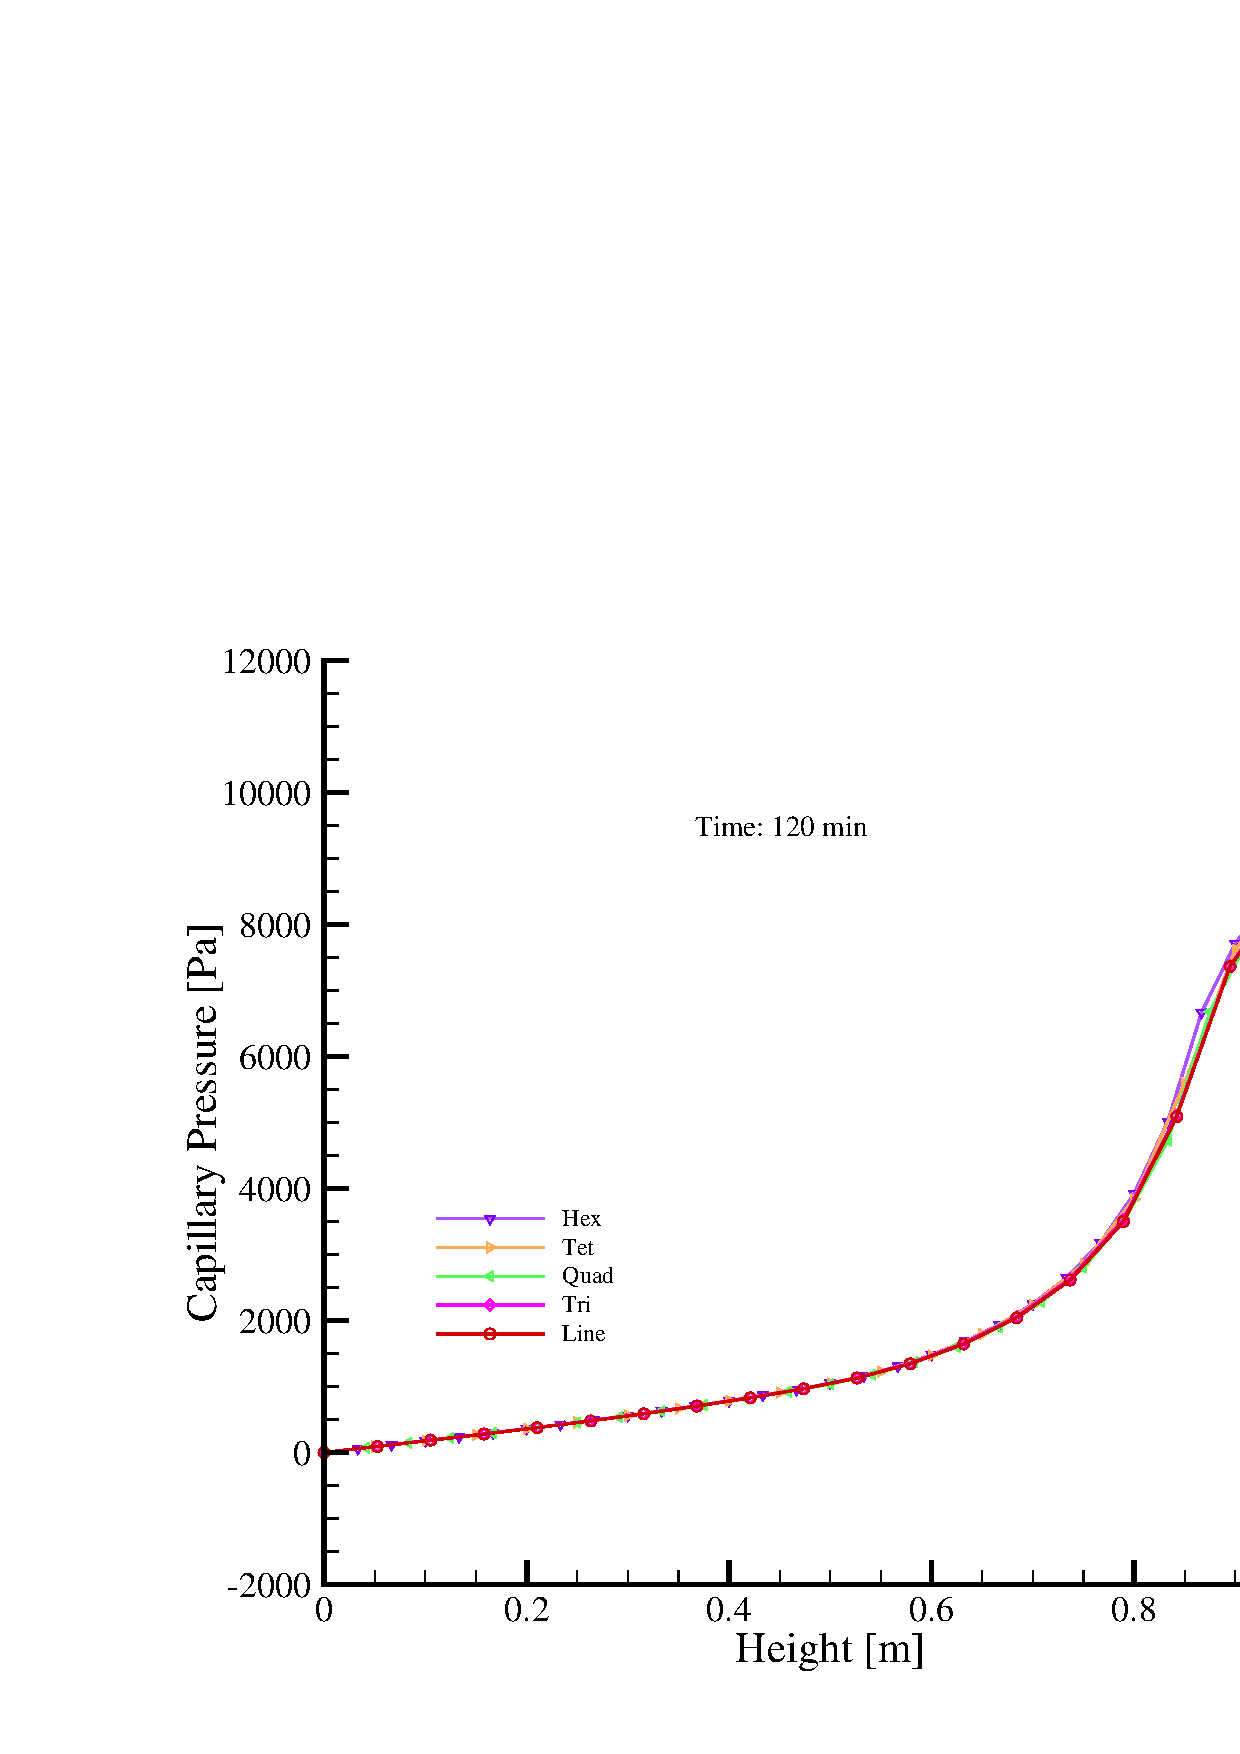
\includegraphics[scale=0.38]{chapter_13/figures/fig_13_1_4}
\end{center}
\caption{Results of element test.}
\label{liak:p_pce}
\end{figure}


%-------------------------------------------------------------------------
\subsection{Buckley-Leverett problem}
Buckley and Leverett \cite{BucLev:1941} developed a semi-analytical solution for the displacement of two immiscible fluids in porous media. Assuming constant fluid density and porosity, and no source/sink terms, the fluid mass balance equation can be simplified to obtain

\begin{equation}
n \frac{\partial S^\gamma }{\partial t} = - \nabla \cdot
\mathbf{q}^\gamma.
\end{equation}

Buckley and Leverett derived the following expression

\begin{equation}
\frac{\partial S^l}{\partial f^l} = \frac{q_{tot}}{n} \frac{\Delta
t}{\Delta x}
\end{equation}

with the fractional flow function $f^\gamma = q^\gamma/q_{tot}$

\begin{equation}
f^1 = \left( 1 + \frac{\mu_1}{k_1} \frac{k_2}{\mu_2} \right)^{-1}
\end{equation}

where 1 and 2 are the fluid phase numbers. The position of the shock front separating the two fluid phases can be calculated from the following expression

\begin{equation}
\Delta x = - \frac{q_{tot}}{n} \frac{\partial f^l}{\partial S^l}.
\end{equation}

Buckley and Leverett suggested that the capillary pressure is a function of the saturation only. Note that the original Buckley-Leverett solution considered phases of water and oil. Moreover, they assumed that the condition that the derivative of the capillary pressure with respect to saturation is zero $(dp_{cwo}/dS_{wo}= 0)$ is a sufficient approximation that both
gradients of water and oil are equal to each other

\begin{equation}
\frac{\partial p_w }{\partial x} = \frac{\partial p_o}{\partial x}
+ \frac{\partial p_{cwo}}{\partial x} = \frac{\partial p_o
}{\partial x} + \frac{dp_{cwo}}{dS^w }\frac{\partial S^w}{\partial
x} = \frac{\partial p_o}{\partial x}.
\end{equation}

\subsubsection*{Definition}
The Buckley Leverett problem is frequently used to test numerical models for the functional relation between relative permeability and saturation. In comparison to the analytical solution, the problem is simplified to describe one fluid displacing the other residing fluid in aquifers or reservoirs. In the derivation of the analytical solution, the effect caused by capillary forces between two fluids is not considered.

A non-wetting phase displaces a wetting phase from left to right. The initial total velocity of the two-phase system is $1.0 m/s$. The ratio of the dynamic viscosities is one, residual saturations are zero and the Brooks-Corey function ($\lambda = 2$) is used for the relative permeabilities. A space-time discretization of delta x = 0.025 m and delta $t = 0.005$. The total simulation time is $0.4 s$.

\begin{figure}[!tbh]
\begin{center}
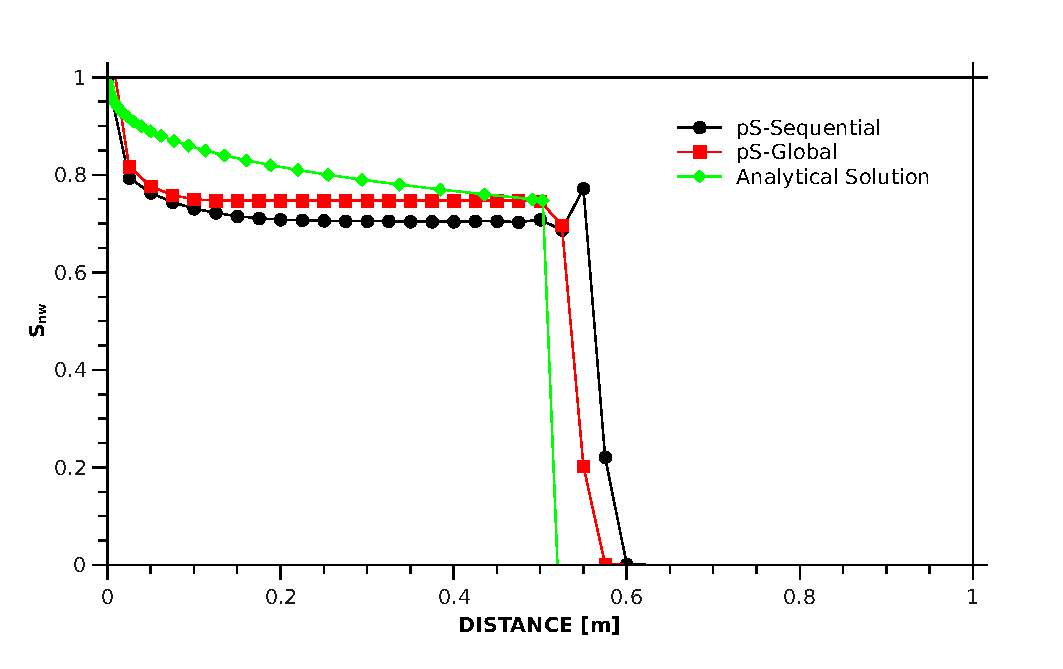
\includegraphics[width=0.8\textwidth]{chapter_13/figures/fig_13_1_5}
\end{center}
\caption{Comparison of coupling schemes and analytical solution for the BL problem.}
\label{blg:comparison}
%\end{figure}
%\begin{figure}[htb]
\begin{center}
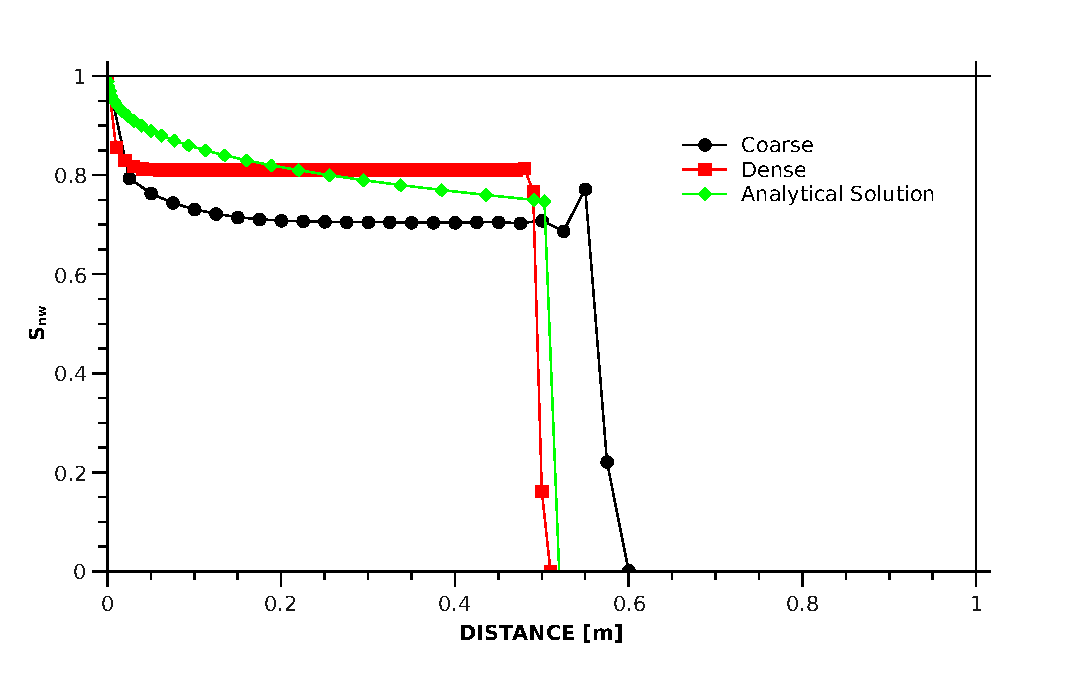
\includegraphics[width=0.8\textwidth]{chapter_13/figures/fig_13_1_6}
\end{center}
\caption{Comparison of grid discretizations for the BL problem with sequential coupling.}
\label{bls:comparison}
\end{figure}

\subsubsection*{Results: pS-Global}
The mass conservation equation is converted to a volumetric one by dividing through by fluid density,

\begin{align}
n\frac{{\partial S_{w}}}{{\partial t }} -
\nabla \cdot \left({\frac{{\mathbf k {k_{rel}}_w }}{{\mu_w }}\left( {\nabla p_w - \rho _w
\mathbf g} \right)} \right) = q_w
\label{eq:w_eqn}
\end{align}
\begin{align}
n\frac{{\partial S_{nw}}}{{\partial t }} -
\nabla \cdot \left({\frac{{\mathbf k {k_{rel}}_{nw} }}{{\mu_{nw} }}\left( {\nabla p_{nw} - \rho _{nw}\mathbf g} \right)} \right) = q_{nw}.
\label{eq:nw_eqn}
\end{align}

In the pressure-saturation scheme, OpenGeoSys solves these two equations in a global-implicit scheme or as a total pressure based sequential coupling. As shown in Fig. \ref{blg:comparison}, the global-implicit scheme produces more accurate result compared to that obtained by the sequential-coupling scheme. The result has little oscillation and is closer to the analytical solution, particularly in the location of the sharp front of the intruding fluid.

One important note is that the global scheme is sensitive to matrix solvers. The LIS solver (BiCG with Jacobi preconditioned) works well on Windows. However, this iterative solver for this benchmark takes much more time than the PARDISO (a parallel direct solver) that works only on Unix with OpenGeoSys.

\subsubsection*{Results: pS-Sequential}
Adding (\ref{eq:w_eqn}) and (\ref{eq:nw_eqn}) and using the relation $S_{nw}+ S_w = 1$ and $p^{c}(S_w) = p_{nw} - p_w$, we get the equation for wetting phase pressure, $p_{w}$ and non-wetting phase saturation, $S_{nw}$.

\begin{align}
 - n\frac{{\partial S_{nw}}}{{\partial t }} -
\nabla \cdot \left({\frac{{\mathbf k {k_{rel}}_w }}{{\mu_w }}\left( {\nabla p_w - \rho _w
\mathbf g} \right)} \right) = q_w
\label{eq:wfn_eqn}
\end{align}
\begin{align}
\nabla \cdot \left({\frac{{\mathbf k {k_{rel}}_w }}{{\mu_w }}\left( {\nabla p_w - \rho _w
\mathbf g} \right)} \right) +
\nabla \cdot \left({\frac{{\mathbf k {k_{rel}}_{nw} }}{{\mu_{nw} }}\left( {\nabla {p_w+p_c} - \rho _{nw}\mathbf g} \right)} \right) + \nonumber\\q_w + q_{nw} =0
\label{eq:nwfn_eqn}
\end{align}

In (\ref{eq:wfn_eqn}), non-wetting phase saturation, $S_{nw}$ can be easily solved explicitly with the known pressure obtained from (\ref{eq:nwfn_eqn}). The analytical solution for the frontal location of the infiltrating fluid is compared with alternate discretizations in Fig. \ref{bls:comparison}. The diffusion term for saturation omitted in the BL equation makes the analytical solution purely advective, with a sharp advancing front. Handling this purely advective transport in numerical models introduces some numerical dispersion, and tighter discretizations will capture the low diffusive front with greater accuracy.

\subsubsection*{Results: $CO_2$ Injection}
Based on the Buckley and Leverett solution, we assume saturated $CO_2$ displacing $H_2O$ with constant fluid properties. Fig. \ref{bl:comparison} shows the saturation profile, $S_w$, along $1~m$ column calculated with line element with space-time discretization of $\delta x = 0.025~m$ and $\delta t = 0.005~s$. The total simulation time is $0.4~s$; using the global implicit pressure-saturation model. Based on linear relation between saturation and relative permeability, the saturation profile, $S_w$ is shown in Fig. \ref{bl:comparison2}.

\begin{figure}[!tbh]
\begin{center}
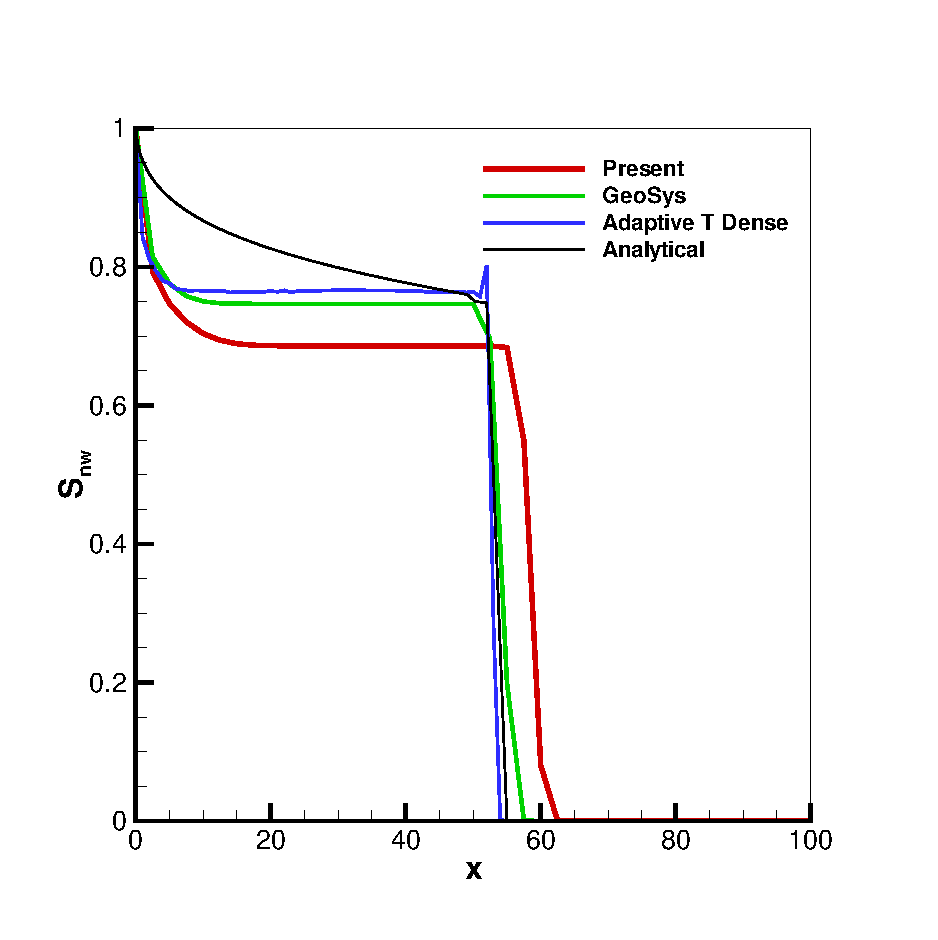
\includegraphics[width=0.6\textwidth]{chapter_13/figures/fig_13_1_7}
\end{center}
\caption{Saturation profile obtained with present analysis along with others.}
\label{bl:comparison}
\end{figure}

\begin{figure}[!tbh]
\begin{center}
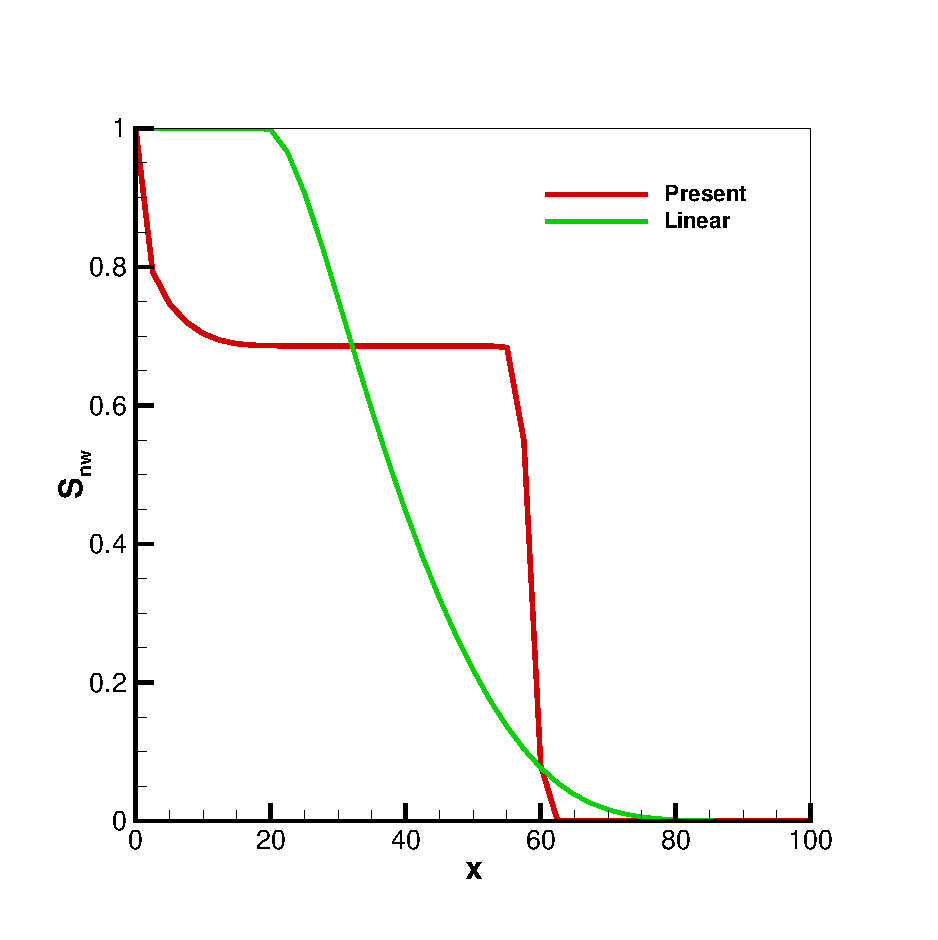
\includegraphics[width=0.6\textwidth]{chapter_13/figures/fig_13_1_8}
\end{center}
\caption{Saturation profile obtained with Brooks-Corey relative permeability function and a linear permeability-saturation function.}
\label{bl:comparison2}
\end{figure}

\begin{table}[!htb]
\begin{tabular}{lccr}
\hline\noalign{\smallskip}
Property & Symbol & Value & Unit \\
\noalign{\smallskip}\hline\noalign{\smallskip}
Column length & $L$ & $m$ & $1.0$  \\
Porosity & $n$ & -- & $2.0\times10^{-1}$ \\
Permeability & $\kappa$ & $ m^2$ & $1.0\times 10^{-10}$ \\
Water dynamic viscosity &  $\mu_w$ & $Pa.s$ & $1.0\times10^{-3}$ \\
Gas dynamic viscosity & $\mu_{nw}$ & $Pa.s$ & $7.0343\times10^{-4}$ \\
Water density &  $\rho_w$ &$kg.m^{-3}$ & $1.0\times10^{3}$ \\
Gas density &  $\rho_{nw}$ & $kg.m^{-3}$ & $7.73\times10^{2}$ \\
Capillary pressure & $p^c(S)$ & $Pa$ & 0 \\
Relative permeability & $\kappa_{rel}(S)$ & -- & Brook-Corey functions \\
\noalign{\smallskip}\hline
\end{tabular}
\caption{Material parameters for the BL problem.}
\end{table}


%-------------------------------------------------------------------------
\subsection{McWhorter problem}

It is assumed that the flow of both wetting and non-wetting phases can be adequately described by Darcy's law if the phases are immiscible and incompressible

\begin{equation}
n\frac{\partial S^{\gamma}}{\partial t} + \nabla \cdot \mathbf{q}^{\gamma} = 0, \gamma=w, nw
\label{eq:mcwtMassEq}
\end{equation}
\begin{equation}
\mathbf{q}^{\gamma}=-{\mathbf K} \lambda^{\gamma} \nabla p^{\gamma}
\label{eq:mcwtFluxEq}
\end{equation}

where $\lambda_w$ and  $\lambda_{nw}$ are mobility of the wetting and non-wetting fluid. Both phase are linked by the state equation $S_w+S_{nw}=1$ and $p_c=p_g-p_w$. Here total flux, $\mathbf {q}_t=\mathbf {q}_w + \mathbf {q}_{nw}$ and $p_c$ is a function of $S_w$.

A formulation that is often used for two phase flow problems is the so-called fractional flow model. The attractiveness of this formulation is that the model becomes more accessible to analysis. Subtracting equation ($18.1.24$) for both phases we have

\begin{equation}
\mathbf {q}_w=f \mathbf {q}_t- D \frac{\partial S_w}{\partial x}
\label{eq:McWhorterWetFlux}
\end{equation}

where 

\begin{equation}
f=\frac{1}{1 + \frac{\lambda_{nw}}{\lambda_w}},~~~D=-\lambda_{nw} f \frac{\partial p_c}{\partial S_w}.
\end{equation}

The first term on the right of equation (\ref{eq:McWhorterWetFlux}) dictates the rate at which flux is injected on the boundary and the second term represent the additional force due to the gradient of capillary pressure. Inserting equation (\ref{eq:McWhorterWetFlux}) into equation (\ref{eq:mcwtMassEq}) for the wetting phase and assuming that total flux, $\mathbf q_t$ is space invariant

\begin{equation}
\frac{\partial }{\partial x}\left( D\frac{\partial S_w}{\partial x}\right) - \mathbf q_t \frac{\partial f}{\partial S_w}\frac{\partial S_w}{\partial x}=n \frac{\partial S_w}{\partial t}.
\label{eq:McWhorterAnal}
\end{equation}

In the last benchmark (Buckley and Leveret) it is assumed that teh force due to the gradient of capillary pressure is very small relative to total flux, $\mathbf q_t$, and hence the second order term is suppressed in the equation.

Including capillarity, model verification can occur against the analytical solution of McWhorter and Sunada ($1990$). They developed an exact quasi-analytical solution of equation (\ref{eq:McWhorterAnal}) for unidirectional displacement of a non-wetting phase by a wetting phase using the concept of a fractional flow function.

The fractional flow function is defined as the ratio of wetting phase flux, $\mathbf q_w$ to the total flux, $\mathbf q_t$. It has been shown that this ratio is function of $S_w$ only, when $\mathbf q_t$ is inversely related to square root of the time.

\subsubsection*{Definition}
The test benchmark problem for capillary effects is formulated as if the instantaneous displacement occurs in a one-dimensional horizontal reservoir initially occupied by oil. Solution has been obtained by solving the governing equations (\ref{eq:msbl_sim}) by the pressure-pressure scheme described above. Different from the Buckley-Leverett problem, here flow is governed by capillary forces when water saturation at the left end of the horizontal column is kept to be one, while the right end is kept to be zero flux. Therefore, no source term exists, and flow is by capillary force alone.

\begin{figure}[!tbh]
\begin{center}
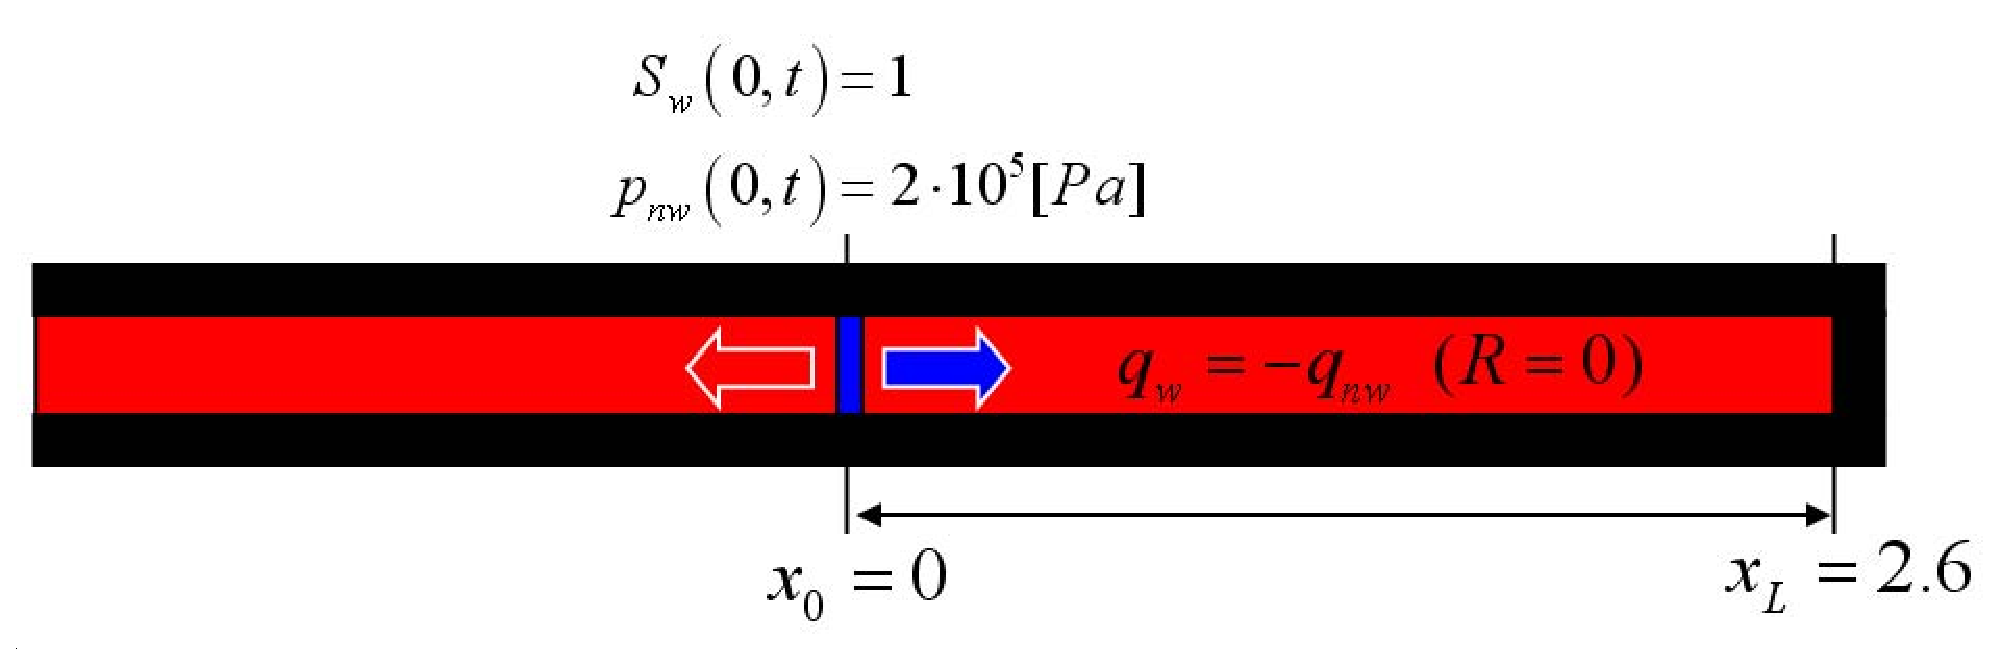
\includegraphics[height=3cm]{chapter_13/figures/fig_13_1_9}
\end{center}
\caption{Schematic of the benchmark formulated to test McWhorter and Sunada's analytical solution.}
\label{mcwt:config}
\end{figure}

\subsubsection*{Results}
Based on the above discussion OpenGeoSys produces an agreeable solution. Fig. \ref{mcwt:ppModel} shows the water saturation profile, $S_w$ with a fine grid along with $2.6m$ long horizontal column for different time steps. Line elements have been used with the time and space discretization $\delta t=0.5s$ and $\delta x=0.05m$ respectively.

\begin{figure}[!tbh]
\begin{center}
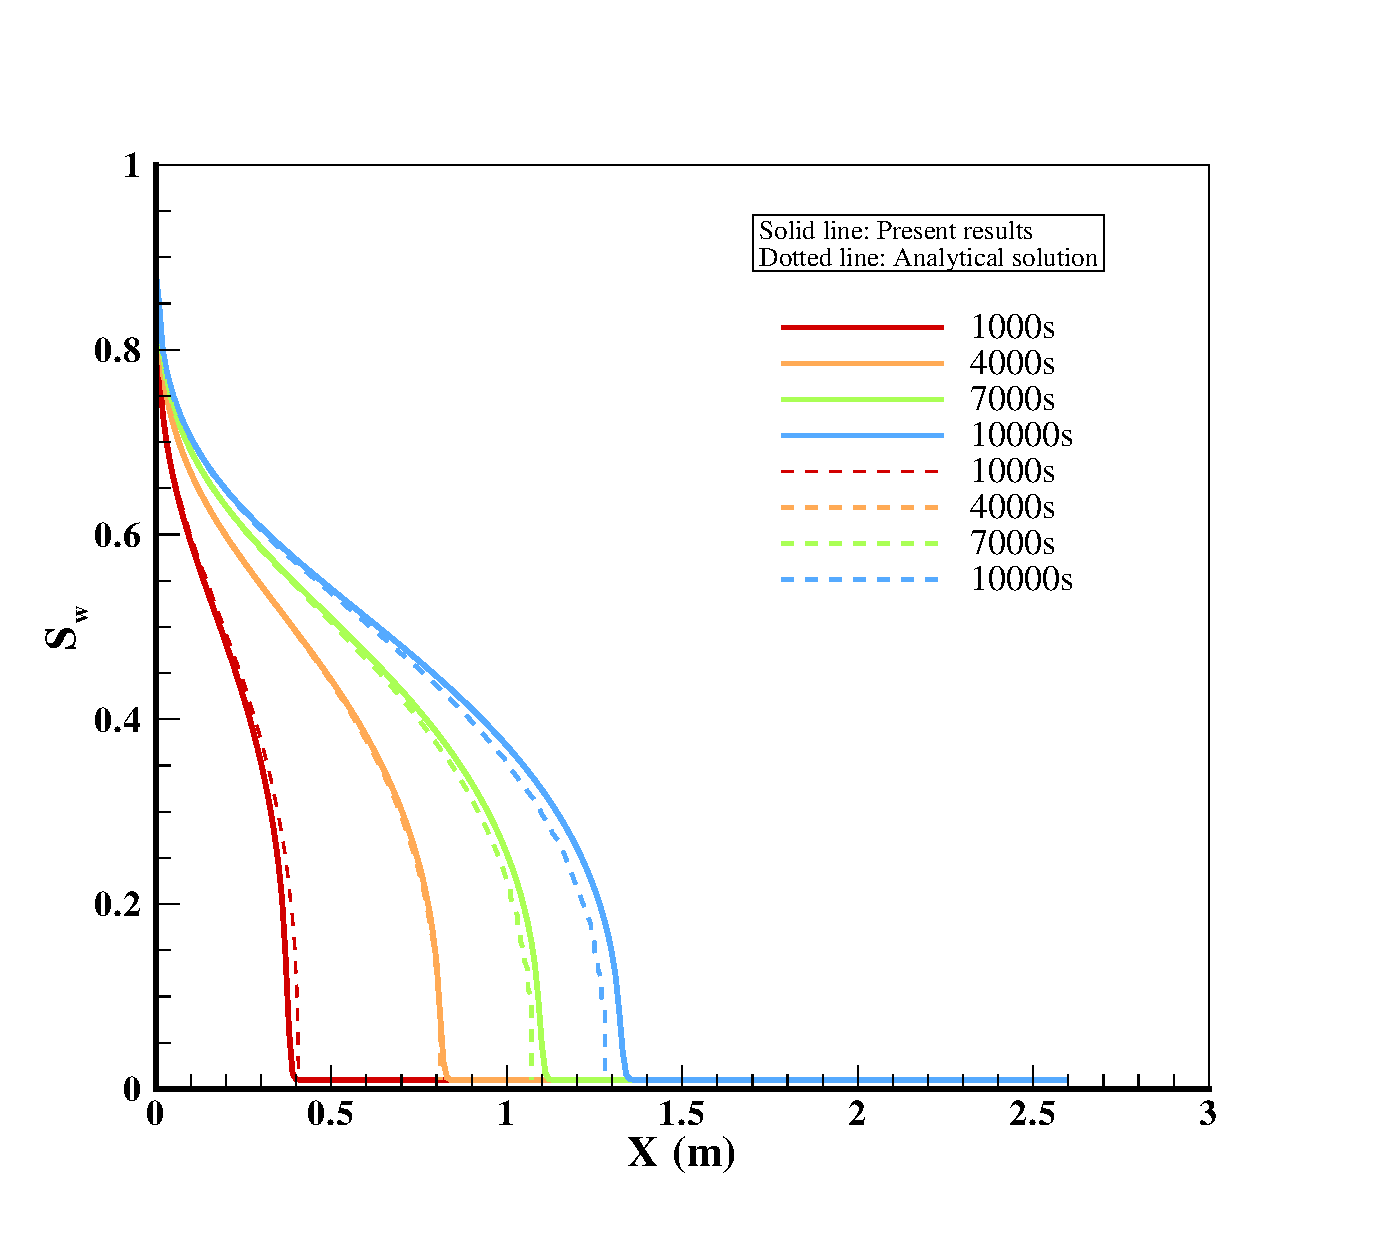
\includegraphics[width=0.7\textwidth]{chapter_13/figures/fig_13_1_10}
\end{center}
\caption{Water saturation, $S_w$ profile of the present result along with analytical solution based on one by McWhorter.}
\label{mcwt:ppModel}
%\end{figure}
%\begin{figure}[!htb]
\begin{center}
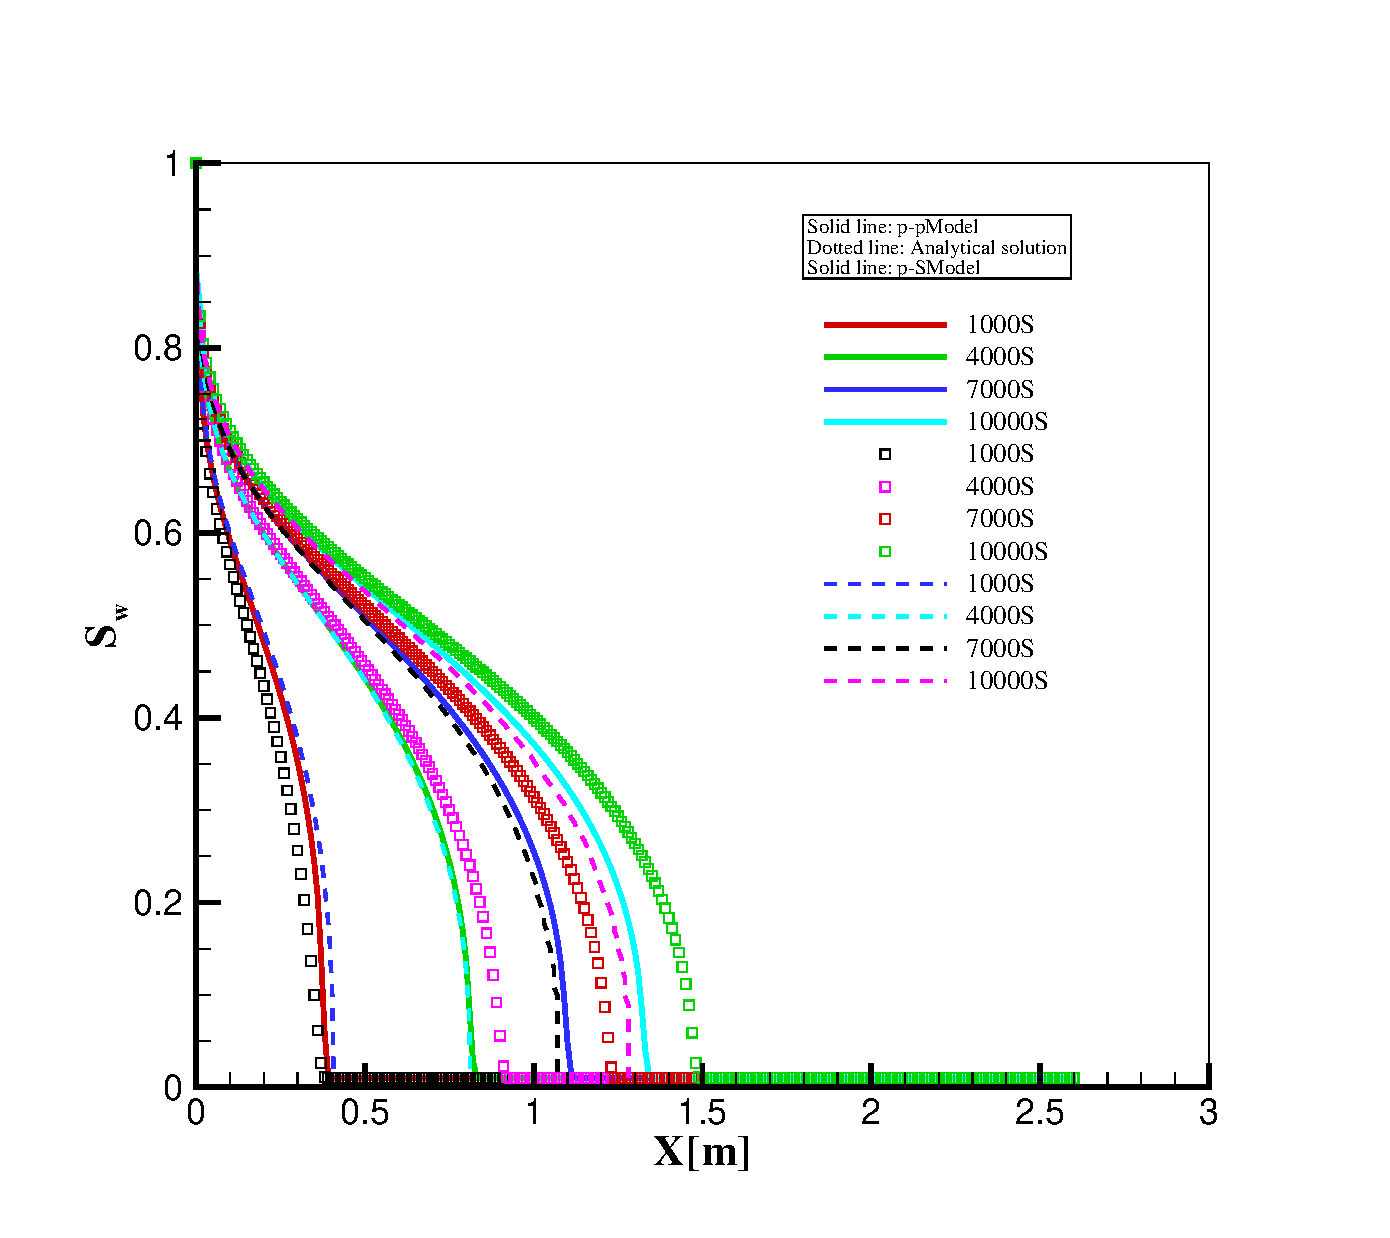
\includegraphics[width=0.7\textwidth]{chapter_13/figures/fig_13_1_11}
\end{center}
\caption{Water saturation, $S_w$ profile in sequential iterative coupling scheme.}
\label{mcwt:psModel}
\end{figure}

Next, we solve exactly same problem using the total pressure based pressure-saturation model in a sequential iterative coupling scheme. Unlike the pressure-pressure model, one downside for the total-pressure-based saturation model is that it is less accurate for problems dominated by capillarity (see Fig. \ref{mcwt:psModel}). Since the pressure-pressure model directly solves for capillary pressure as a primary variable, the model has an advantage for the capillary related problems. On the other hand, the total-pressure-based saturation model is limited to the problems when $d P_c/d S_w$ is close to zero. The condition for $d P_c/d S_w$ close to zero is caused physically in the case of fractures, shear zones, and transitions between heterogeneities.

\begin{table}[!htb]
\begin{tabular}{lccr}
\hline\noalign{\smallskip}
Property & Symbol & Value & Unit \\
\noalign{\smallskip}\hline\noalign{\smallskip}
Column length & $L$ & $m$ & $2.6$  \\
wetting dynamic viscosity &  $\mu_w$ & $Pa.s$ & $1.0\times10^{-3}$ \\
non-wetting dynamic viscosity & $\mu_{nw}$ & $Pa.s$ & $1.0\times10^{-3}$ \\
wetting phase density &  $\rho_w$ &$kg.m^{-3}$ & $1.0\times10^{3}$ \\
Non-wetting phase density &  $\rho_{nw}$ & $kg.m^{-3}$ & $1.0\times10^{3}$ \\
Permeability & $\mathbf K$ & $ m^2$ & $1.0\times 10^{-10}$ \\
Porosity & $n$ & $--$ & $3.0\times10^{-1}$ \\
Residual saturation of water &  $S_{rw}$ & $--$ & $0$ \\
Residual saturation of oil &  $S_{nrw}$ & $--$ & $0$ \\
Entry pressure &  $p_d$ & $Pa$ & $5.0\times10^{3}$ \\
Soil distribution index &  $\lambda$ & $--$ & $2.0$ \\
Capillary pressure & $p^c(S_{eff})$ & $Pa$ & Brooks-Corey model\\
Relative permeability & $\kappa_{rel}(S_{eff})$ & $--$ & Brooks-Corey model \\
\noalign{\smallskip}\hline
\end{tabular}
\caption{Material parameters for the McWhorter problem.}
\end{table}

%-------------------------------------------------------------------------
\subsection{Kueper problem}
Both primary variable schemes are now further tested with a benchmark chosen to examine two-phase flow in heterogeneous media. Kueper and Frind (1991) developed a model to simulate their experiment for DNAPL penetration (Kueper et al., $1989$). The simultaneous movement of a dense non-wetting phase (DNAPL) through an initially wetting phase (water) saturated heterogeneous porous media may be represented mathematically as a case of two-phase flow. A distinctive feature of the solution is that the primary variables solved for, wetting phase pressure and wetting phase saturation, are both existent throughout the solution domain regardless of whether the non-wetting phase is present.

The continuity equation of each phase ($\gamma$) can be defined by
\begin{equation}
\frac{\partial (n {\rho}^{\gamma} S^{\gamma})}{\partial t} + \nabla \cdot ({\rho}^{\gamma} \mathbf{q}^{\gamma}) = \mathbf{Q}^{\gamma}, \gamma=w, nw
\label{eq:mcwtMassEq}
\end{equation}
where $n$ is porosity, $S^{\gamma}$ is saturation, $\rho^{\gamma}$ is density, $\mathbf{Q}^{\gamma}$ is a source or sink term, and $\mathbf{q}^{\gamma}$ is the Darcy velocity for phase $\gamma$ defined by
\begin{equation}
\mathbf{q}^{\gamma}=-{\mathbf K} \frac{\kappa_r^{\gamma}}{\mu^{\gamma}}(\nabla p^{\gamma}-{\rho}^{\gamma} \mathbf{g}), \gamma=w, nw
\label{eq:mcwtFluxEq}
\end{equation}

where $\kappa_r^{\gamma}$ is relative permeability, $\mu^{\gamma}$ is viscosity, $p^{\gamma}$ is pressure for phase $\gamma$, $\textbf{K}$ is intrinsic permeability tensor and $\mathbf{g}$ is the gravitational vector.  

Inherently for saturation, the sum of all saturation in pore space is

\begin{equation}
{\sum S^{\gamma}}=1.
\label{eq:mcwtFluxEq}
\end{equation}

Assuming relative preference (i.e., wettability) of the fluid to media exists and it is not negligible, the capillary pressures relation for a two-phase system is defined over representative elementary volume (REV) by 

\begin{equation}
p_c=p_{nw}-p_w
\label{eq:mcwtFluxEq}
\end{equation}                                                 
where $p_c$ is capillary pressure, $p_{nw}$ is pressure for the non-wetting phase fluid and $p_w$ is the wetting phase fluid. 

\begin{figure}[!tbh]
\begin{center}
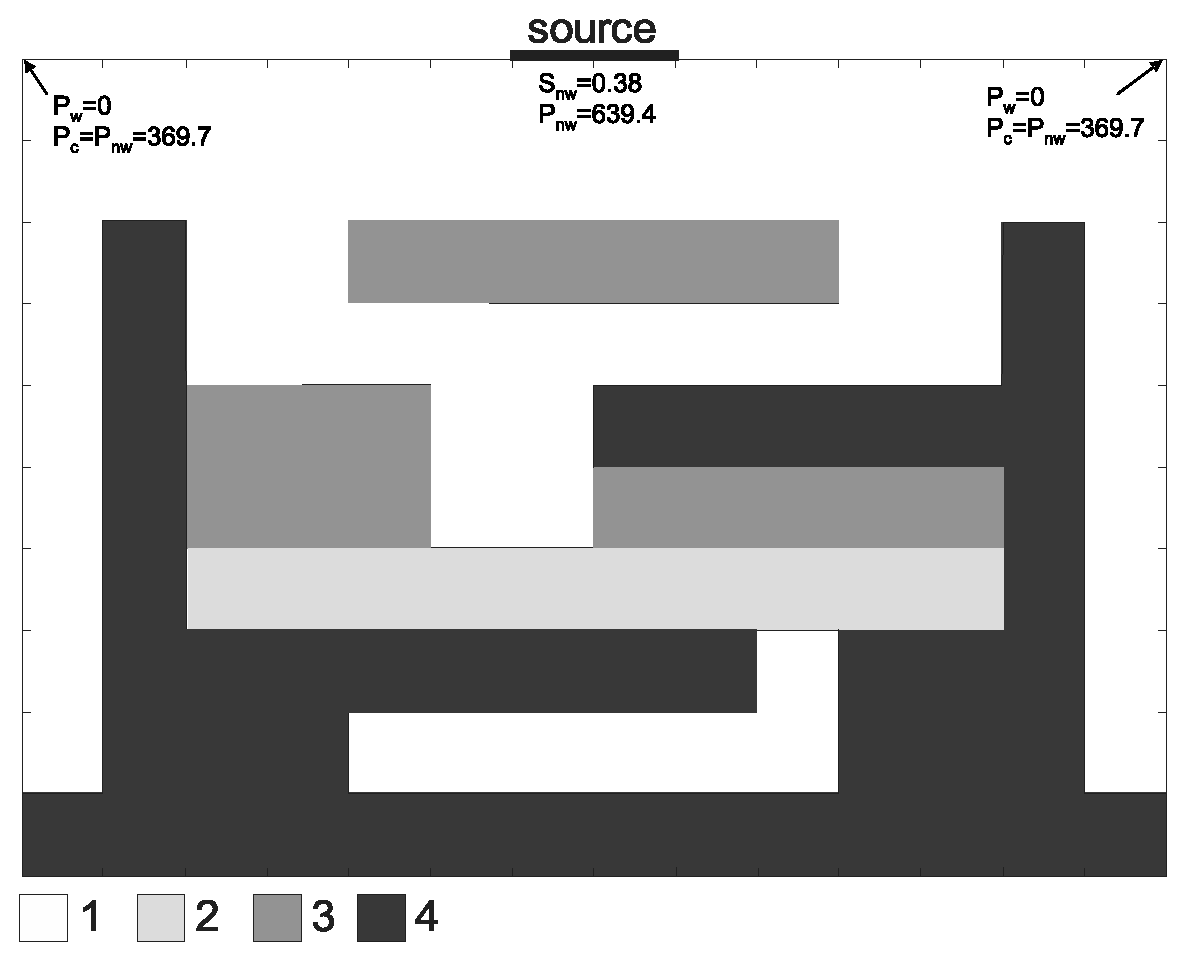
\includegraphics[height=5cm]{chapter_13/figures/fig_13_1_12}
\end{center}
\caption{Configuration of heterogeneous media in parallel-plate cell.}
\label{mcwt:keuperconfig}
\end{figure}

\subsubsection*{Definition}
A $60cm\times80cm\times0.6cm$ parallel-plate glass-lined cell was packed with four types of sands and initially fully saturated with water. The configuration of the assembled sand lenses and the two sets of the boundary conditions for the $p_w-S_{nw}$ and $p_c-p_{nw}$ schemes are illustrated in Fig. \ref{mcwt:keuperconfig}. Concerning to the constitutive relation between relative permeability and saturation and capillary pressure and saturation, they have used the Brooks-Corey model. 

Properties of sands for the Brooks-Corey model are measured experimentally and summarized in the following tables. The numerical solutions obtained from the $p_w-S_{nw}$ scheme and the $p_c-p_{nw}$ scheme for the benchmark Kueper and Frind ($1991$) are compared against each other in Fig. \ref{mcwt:keuperresults}. 

\begin{table}[!htb]
\begin{center}
\begin{tabular}{lccc}
\hline
Fluid properties & Unit & Wetting fluid	& Non-wetting fluid \\
\hline
Density &	$kg.m^{-3}$ &	$1.0\times10^3$ &	$1.0\times10^3$ \\ 
Viscosity &	$Pa\cdots$ & $1.0\times10^{-3}$ &	$1.0\times10^{-3}$ \\
Residual saturation &	- &	0.0 &	0.0 \\
Maximum saturation &	- &	1.0 &	1.0 \\
\hline
\end{tabular}
\caption{Fluid and medium properties.}
\end{center}
\end{table}

\begin{table}[!htb]
\begin{center}
\begin{tabular}{lcc}
\hline
Medium properties & Unit & Medium\\
\hline
$\Delta x$ & m &	0.01 \\
$\Delta t$ & s &	100 \\
Porosity & - &	0.3 \\
Intrinsic permeability & $m^2$ & $1\times10^{-10}$ \\
Brook-Corey's index &	- &	2 \\
Entry pressure & Pa & $5\times10^3$ \\
\hline
\end{tabular}
\caption{Space and time discretization.}
\end{center}
\end{table}

\begin{table}[!htb]
\begin{center}
\begin{tabular}{lccccc}
\hline
Property & $P_d$(Pa) & $\lambda$(-) &	$S_{wr}$(-) &	k($m^2$) &	$n$(-) \\
\hline
1	& 369.73 & 3.86	& 0.078	& $5.04\times10^{-10}$ & 0.40 \\ 
2	& 434.45 & 3.51 & 0.069 &	$2.05\times10^{-10}$ & 0.39 \\
3	& 1323.95 &	2.49 & 0.098 &	$5.26\times10^{-11}$ & 0.39 \\
4	& 3246.15	& 3.30 & 0.189 & $8.19\times10^{-12}$ &	0.41 \\
\hline
\end{tabular}
\caption{Hydraulic properties of sands for the Brooks-Corey model.}
\end{center}
\end{table}

\subsubsection*{Results}
Both schemes produce DNAPL plume propagation physically until the plume reaches the less permeable media under the top medium in the model domain. The striking difference occurs at the interface between these two media. While the pwSnw scheme simulates the plume to infiltrate into the less previous medium, the $p_c-p_{nw}$ scheme forces the plume to bypass the less previous medium. A similar experiment and simulation comparison against experimental observation are also conducted by Helming and Huber ($1998$). They have reported unphysical fluid behavior captured by the $p_w-S_{nw}$ scheme, a phenomenon that can be avoided with fully upwind technique (Helming and Huber, $1998$). 

\begin{figure}[!tbh]
\begin{center}
\includegraphics[width=1.0\textwidth]{chapter_13/figures/fig_13_1_13}
\end{center}
\caption{Comparison of the results obtained from the $p_w-S_{nw}$ and $p_c-p_{nw}$ schemes. The second column shows good agreement with observed distribution of DNAPL of the experiment (Kueper and Frind $1991$).}
\label{mcwt:keuperresults}
\end{figure}












